\documentclass[italian]{article}
\usepackage[T1]{fontenc}
\usepackage[utf8]{inputenc}
\usepackage{lmodern}
\usepackage{hyperref}
\usepackage[a4paper,top=3cm,bottom=3cm,left=2.5cm,right=2.5cm]{geometry}
\usepackage[italian]{babel}
\usepackage{listings} %Per inserire codice
\usepackage[usenames]{color} %Per permettere la colorazione dei caratteri 
%Define the listing package
\usepackage{listings} %code highlighter
\usepackage{color} %use color
\usepackage{graphicx}
\graphicspath{ {./images/} }
\definecolor{mygreen}{rgb}{0,0.6,0}
\definecolor{mygray}{rgb}{0.5,0.5,0.5}
\definecolor{mymauve}{rgb}{0.58,0,0.82}

%Customize a bit the look
\lstset{ %
	backgroundcolor=\color{white}, % choose the background color; you must add \usepackage{color} or \usepackage{xcolor}
	basicstyle=\footnotesize, % the size of the fonts that are used for the code
	breakatwhitespace=false, % sets if automatic breaks should only happen at whitespace
	breaklines=true, % sets automatic line breaking
	captionpos=b, % sets the caption-position to bottom
	commentstyle=\color{mygreen}, % comment style
	deletekeywords={...}, % if you want to delete keywords from the given language
	escapeinside={\%*}{*)}, % if you want to add LaTeX within your code
	extendedchars=true, % lets you use non-ASCII characters; for 8-bits encodings only, does not work with UTF-8
	frame=single, % adds a frame around the code
	keepspaces=true, % keeps spaces in text, useful for keeping indentation of code (possibly needs columns=flexible)
	keywordstyle=\color{blue}, % keyword style
	% language=Octave, % the language of the code
	morekeywords={*,...}, % if you want to add more keywords to the set
	numbers=left, % where to put the line-numbers; possible values are (none, left, right)
	numbersep=5pt, % how far the line-numbers are from the code
	numberstyle=\tiny\color{mygray}, % the style that is used for the line-numbers
	rulecolor=\color{black}, % if not set, the frame-color may be changed on line-breaks within not-black text (e.g. comments (green here))
	showspaces=false, % show spaces everywhere adding particular underscores; it overrides 'showstringspaces'
	showstringspaces=false, % underline spaces within strings only
	showtabs=false, % show tabs within strings adding particular underscores
	stepnumber=1, % the step between two line-numbers. If it's 1, each line will be numbered
	stringstyle=\color{mymauve}, % string literal style
	tabsize=2, % sets default tabsize to 2 spaces
	title=\lstname % show the filename of files included with \lstinputlisting; also try caption instead of title
}
%END of listing package%

\definecolor{darkgray}{rgb}{.4,.4,.4}
\definecolor{purple}{rgb}{0.65, 0.12, 0.82}

%define Javascript language
\lstdefinelanguage{JavaScript}{
	keywords={typeof, new, true, false, catch, function, return, null, catch, switch, var, if, in, while, do, else, case, break},
	keywordstyle=\color{blue}\bfseries,
	ndkeywords={class, export, boolean, throw, implements, import, this},
	ndkeywordstyle=\color{darkgray}\bfseries,
	identifierstyle=\color{black},
	sensitive=false,
	comment=[l]{//},
	morecomment=[s]{/*}{*/},
	commentstyle=\color{purple}\ttfamily,
	stringstyle=\color{red}\ttfamily,
	morestring=[b]',
	morestring=[b]"
}

\lstset{
	language=JavaScript,
	extendedchars=true,
	basicstyle=\footnotesize\ttfamily,
	showstringspaces=false,
	showspaces=false,
	numbers=left,
	numberstyle=\footnotesize,
	numbersep=9pt,
	tabsize=2,
	breaklines=true,
	showtabs=false,
	captionpos=b
}
\author{
	Daniele Rigon - 857319 \\
}


\begin{document}
	
	\title{Tesi - Payment Request API}
	\maketitle
	
	\tableofcontents
	\pagebreak
	
	\section{Overview Payment Request}
	Fare acquisti sul web, in particolare sui dispositivi mobili, può essere un'esperienza frustrante, in quanto ogni sito Web ha il proprio sistema e la maggior parte dei siti richiede agli utenti di digitare manualmente le stesse informazioni (di contatto, credenziali di pagamento, indirizzi) più e più volte, e questa ridondanza può portare alla perdita di clienti.
	Allo stesso modo creare e gestire pagine che supportano diversi meotodi di pagamanto puo risultare difficile, e puo richiedere molto tempo agli sviluppatori.
	La PaymentRequest API consente ai commercianti di creare esperienze di pagamento semplificate. Piuttosto che ridigitare le stesse informazioni più volte nel Web, gli utenti possono memorizzare e riutilizzare le informazioni e completare più rapidamente e accuratamente le transazioni online.
	
	\subsection{Concetti e utilizzo della richiesta di pagamento}
	
	Molti problemi legati all'abbandono degli acquisti online possono essere ricondotti ai moduli di checkout, difficili da usare, lenti da caricare e aggiornare e richiedono più passaggi da completare. La PaymentRequest API è un sistema che ha lo scopo di eliminare i moduli di checkout, migliorando il flusso di lavoro degli utenti durante il processo di acquisto, offrendo un'esperienza utente più coerente e consentendo ai commercianti di sfruttare facilmente diversi metodi di pagamento. 
	
	\subsection{Vantaggi nell'utilizzo di questa API}
	\begin{itemize}
	\item Esperienza di acquisto rapida: gli utenti immettono i propri dati una volta nel browser e sono pronti a pagare beni e servizi sul Web; una volta inseriti i dati non è più necessario compilare ripetutamente gli stessi dettagli su siti diversi;
	\item Esperienza coerente su ogni sito (che supporta l'API):  poiché la pagina di pagamento è controllata dal browser si può personalizzare l'esperienza utente, ad esempio includendo la localizzazione per impostare automaticamente la lingua preferita dell'utente, ecc;
	\item Gestione delle credenziali: gli utenti possono gestire le loro carte di credito e gli indirizzi di spedizione direttamente nel browser. Un browser può anche sincronizzare queste "credenziali" tra dispositivi, rendendo più semplice per gli utenti passare dal desktop al cellulare e viceversa quando si acquistano oggetti;
	\item Gestione coerente degli errori: il browser può controllare la validità dei numeri delle carte e può comunicare all'utente se una carta è scaduta o sta per scadere, può suggerire automaticamente quale carta utilizzare in base ai modelli di utilizzo passati o alle restrizioni del commerciante, o consentire all'utente di dire quale sia la carta predefinita/preferita.
	\item Esperienza utente migliorata: meno tipizzazione, coerenza tra i siti Web, coerenza tra browser e sistemi operativi e nuove funzionalità del browser per semplificare il checkout, ecc;
	\item Miglioramento della sicurezza: la PaymentRequest API ha il potenziale per ridurre le opportunità di frode e può facilitare l'adozione di metodi di pagamento più sicuri;
	\item Responsabilità inferiore: in passato, per creare un'esperienza utente semplificata, i commercianti dovevano memorizzare le credenziali di pagamento degli utenti. Questo non è più necessario, il che può aiutare a ridurre la responsabilità del commerciante nei confronti del cliente;
	\end{itemize}
	
	\subsection{Come funziona}	
	L'API di richiesta di pagamento consente a un utente di completare una transazione più facilmente riutilizzando le informazioni memorizzate nel browser o in app di pagamento di terze parti.
	Quando l'utente preme un pulsante in una pagina di checkout collegata all'API il commerciante utilizza l'API per richiedere il pagamento. Il commerciante fornisce informazioni su prezzo, valuta e un elenco di metodi di pagamento accettati, e può inoltre richiedere al browser di creare un'interfaccia utente semplificata per raccogliere l'indirizzo di spedizione, le informazioni di contatto e un numero limitato di elementi aggiuntivi dall'utente.
	Il browser determina quali metodi di pagamento sono supportati dal commerciante tra le varie "app di pagamento" mostrandole all'utente. 
	L'utente seleziona un'app di pagamento con la quale pagare, la quale può comportare ulteriori interazioni con l'utente (ad esempio per l'autenticazione); al completamento l'app di pagamento restituisce i dati tramite l'API al commerciante.

	\begin{figure}[h]
		\centering
		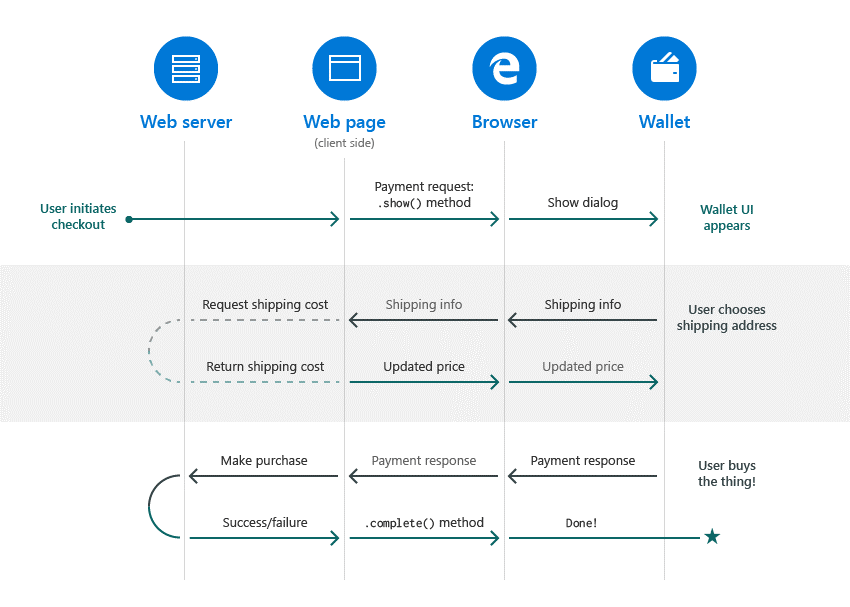
\includegraphics[width=1\linewidth]{SchemaPayment}
		\caption{Schema Payment Request API}
		\label{fig:Schema Payment}
	\end{figure}
	
	\subsection{Rischi}
	La PaymentRequest API consente ai commercianti di "consegnare" la raccolta di credenziali di pagamento alle app di pagamento, riducendo cosi l'onere di creare un'esperienza di pagamento adeguata per l'utente. 
	
	\subsection{Sicurezza API}
	La PaymentRequest API aumenta la sicurezza poichè:
	\begin{itemize}
	\item I commercianti possono ottenere un checkout semplificato senza memorizzare le credenziali dell'utente, in quanto lo fa l'API, rendendo i commercianti meno vulnerabili agli attacchi;
	\item La PaymentRequest API dovrebbe facilitare l'introduzione di metodi di pagamento più sicuri sul Web, come i pagamenti con carta tokenizzata;
	\item I proprietari dei metodi di pagamento disporranno di meccanismi standard per autorizzare software specifici a implementare il loro metodo di pagamento, che il browser può verificare attraverso una firma digitale.
	\end{itemize}
	I browser utilizzano una varietà di meccanismi per archiviare informazioni sensibili dell'utente, e attualmente W3C sta sviluppando nuove tecnologie per aumentarne la sicurezza.
	Per quanto riguarda la memorizzazione delle informazioni delle app di pagamento in modo sicuro, questo è un dettaglio di implementazione che è diverso per ogni app di pagamento, e tale sicurezza è a carico del provider dell'app di pagamento.
	
	\subsection{Uso API}
	\subsubsection{Ruolo dell'utente}
	Gli utenti beneficiano del riutilizzo delle credenziali inserite nel browser o nelle app di pagamento. Quindi, quando si visita un sito Web che sfrutta la PaymentRequest API gli utenti avranno l'opportunità di sfruttare il riutilizzo semplificato delle credenziali archiviate.

	\subsubsection{Ruolo del commerciante}
	L'API influisce sul front end e non sul back-end, ovvero solamente sull'intrfaccia dell'esperienza utente; pertanto il commerciante non dovrebbe dover apportare modifiche all'elaborazione back-end di vari metodi di pagamento, questo sarà compito del fornitore della pagina di pagamento, il quale sostituirà i moduli Web con le chiamate alla PaymentRequest API.
	
	È richiesto il gesto dell'utente per attivare l'API di richiesta di pagamento attraverso PaymentRequest.show().
	
	L'API non include l'autenticazione dell'utente, ma esistono due tipi di autenticazione utente che esulano dall'ambito delle specifiche della PaymentRequest API:
	\begin{itemize}
	\item Autenticazione del commerciante dell'utente: l'utente accede al proprio account con il commerciante;
	\item Autenticazione delle app di pagamento dell'utente: fornendo un codice CVV, tramite nome/password o tramite autenticazione a più fattori.
	\end{itemize}
	
	\subsubsection{Ruolo del browser}
	Il browser svolge diversi ruoli:
	\begin{itemize}
	\item Calcola l'intersezione dei metodi di pagamento accettati dal commerciante e registrati dall'utente;
	\item Visualizza l'interfaccia utente che consente all'utente di inserire le proprie informazioni;
	\item Funge da canale per i dati da e verso il commerciante e da e verso l'utente.
	\end{itemize}
	
	\subsubsection{Metodi di pagamento}
	La PaymentRequest API è progettata per funzionare con un gran numero di metodi di pagamento, i quali vengono identificati attraverso due strade:
	\begin{itemize}
		\item I metodi di pagamento definiti da W3C sono identificati come "basic-card" e sono composti da stringhe corte;
		\item I metodi di pagamento definiti da altre parti sono identificati dagli URL.
	\end{itemize}
	
	\subsubsection{App di pagamento}
	In base alla progettazione,le app di pagamento sono app native per dispositivi mobili e app Web. Il gruppo di lavoro Web Payments sta lavorando su una specifica per come le applicazioni Web si registrano per gestire le richieste di pagamento. Il gruppo di lavoro Web Payments non discute l'integrazione di app di pagamento native su piattaforme proprietarie; che viene gestito dai proprietari di quelle piattaforme.
	Il gruppo di lavoro Web Payments sta sviluppando una specifica che definisce il modo in cui il browser possa sapere quali app di pagamento ha l'utente. L'obiettivo del gruppo di lavoro Web Payments è stabilire un meccanismo di registrazione unico per i programmi utente su qualsiasi sistema.
	Per le app di pagamento create con tecnologia nativa (proprietaria), il browser o il sistema operativo sottostante determinano il meccanismo di registrazione e possono variare da sistema a sistema.
	L'API di richiesta di pagamento, ovvero il browser, determina se un'app di pagamento "corrisponde" a una determinata transazione definendo un algoritmo che considera:
	\begin{itemize}
	\item Se l'app di pagamento supporta uno qualsiasi dei metodi di pagamento accettati dal commerciante. Il commerciante dichiara quali metodi di pagamento supporta attraverso un elenco di identificativi del metodo di pagamento passati attraverso l'API.
	\item Inoltre, alcuni metodi di pagamento consentono ai commercianti e alle app di pagamento di descrivere più dettagliatamente le condizioni in base alle quali accettano o supportano tali metodi di pagamento. Questa informazione di "capacità" viene anche utilizzata per determinare se un'app di pagamento corrisponde a una determinata transazione.
	\end{itemize}
	Al fine di proteggere la privacy degli utenti, i commercianti hanno accesso a informazioni molto limitate sull'ambiente dell'utente. L'API di richiesta di pagamento supporta un meccanismo di query limitato per consentire al commerciante di determinare se l'utente ha "qualcosa" che può essere utilizzato con l'API di richiesta di pagamento, ma che non fornisce informazioni su software specifico. Questa informazione consente ai commercianti di rilevare il supporto per l'API di richiesta di pagamento e quindi di mostrare una pagina di checkout che utilizza l'API, oppure di creare una pagina di fallback se l'utente non è pronto a pagare con qualche app di pagamento.
	I commercianti possono semplificare le pagine di pagamento in diversi modi, tra cui:
	\begin{itemize}
	\item Non avranno bisogno di usare la pagina di checkout per raccogliere la spedizione e altri dati comuni; il browser può fornirlo più rapidamente se l'utente lo ha già archiviato.
	\item Non avranno bisogno di chiedere agli utenti di scegliere un metodo di pagamento. Invece, possono fornire un singolo pulsante che consente al browser di visualizzare app di pagamento rilevanti.
	\end{itemize}
	
	In che modo l'API di richiesta di pagamento influisce sul flusso dei metodi di pagamento che già supporta?
	Oggi, il flusso per gli utenti di solito implica qualcosa del genere:
	\begin{itemize}
	\item Scansione di un elenco di metodi di pagamento accettati (non di cui l'utente si preoccupa)
	\item Scegline uno e continua
	\item Per i metodi di pagamento che prevedono il lancio di un'app o la visita a un sito Web, inviare l'utente a quell'app o sito, quindi inviarli di nuovo dopo che il pagamento è stato completato.
	\end{itemize}
	L'API di richiesta di pagamento consente un flusso migliorato:
	\begin{itemize}
	\item L'utente preme un pulsante di acquisto singolo (non è richiesta alcuna scansione)
	\item Il browser visualizza le app di pagamento dell'utente che possono essere utilizzate per la transazione. È probabile che i browser supportino le preferenze dell'utente in modo che, ad esempio, un'app di pagamento venga avviata automaticamente su un determinato sito Web. Ciò semplificherà ulteriormente il checkout.
	\item Per i metodi di pagamento che prevedono il lancio di un'app o la visita a un sito Web, inviare l'utente a quell'app o sito, quindi inviarli di nuovo dopo che il pagamento è stato completato. Il gruppo di lavoro Web Payments sta discutendo, tuttavia, come possiamo migliorare l'esperienza dell'utente creando un senso più forte di "essere ancora nel contesto commerciale" quando si utilizza un'app o un sito Web da pagare. Più lavoro deve essere fatto su questo argomento.
	\end{itemize}
	
	
	\subsubsection{Differenze tra metodo di pagamento e app di pagamento}
	Nell'ecosistema dell'API della richiesta di pagamento, disaccoppiamo i dati necessari per effettuare un pagamento dal software utilizzato per raccogliere tali dati e avviare l'elaborazione dei pagamenti.
	Un metodo di pagamento è caratterizzato dai dati che il commerciante fornisce al pagatore e riceve dal pagatore per essere pagato.
	\begin{itemize}
	\item Esempio: per un metodo di pagamento con carta di base, il commerciante non fornisce dati al pagatore e riceve dal numero di carta del pagatore, dalla data di scadenza, ecc.
	\item Esempio: per un metodo di pagamento con trasferimento di credito, il commerciante fornisce informazioni sull'account commerciante, ecc. E riceve dalle informazioni del pagatore sulla data di elaborazione, i codici di transazione, ecc.
	\end{itemize}
	Un'app di pagamento è il software che l'utente utilizza per pagare. Un'app di pagamento può supportare uno o più metodi di pagamento. Le app di pagamento possono essere implementate utilizzando una varietà di tecnologie, incluse quelle di sistemi operativi nativi o tecnologie Web o di un ibrido. I browser possono anche fungere da app di pagamento, memorizzando le credenziali dell'utente come le informazioni sulla carta. L'API di richiesta di pagamento e l'API di pagamento non risolvono il funzionamento interno delle app di pagamento, ma solo il modo in cui comunicano con il browser.
	In generale, più app di pagamento possono implementare lo stesso metodo di pagamento. Tuttavia, vi sono casi importanti in cui è disponibile una sola app di pagamento autorizzata a supportare un metodo di pagamento (proprietario).
	Nei casi in cui più app di pagamento possono servire un determinato metodo di pagamento (ad es. "Carta base"), il commerciante non deve preoccuparsi dell'integrazione software. Il commerciante richiede " dati" attraverso l'API di richiesta di pagamento. Il commerciante (o il suo fornitore di servizi di pagamento) deve gestire tali dati sul back-end, ma non è necessaria alcuna integrazione software aggiuntiva. Allo stesso modo, il disaccoppiamento libera l'utente a scegliere la sua app di pagamento preferita.
	

	
	
	\section{Specifiche}
	\subsection{Metodi}
	Per utilizzare l'API, lo sviluppatore deve fornire e tenere traccia di una serie di informazioni chiave. Questi bit di informazioni vengono passati al costruttore PaymentRequest come argomenti e successivamente utilizzati per aggiornare la richiesta di pagamento visualizzata all'utente. Vale a dire, questi bit di informazione sono:
	\begin{itemize}
	\item Il methodData: Una sequenza di PaymentMethodData che rappresenta i metodi di pagamento che il sito supporta;
	\item I details: i dettagli della transazione, come un PaymentDetailsInit. Ciò include il costo totale e facoltativamente un elenco di beni o servizi acquistati, beni materiali e opzioni di spedizione. Inoltre, può facoltativamente includere "modificatori" su come vengono effettuati i pagamenti. Ad esempio, "se paghi con una carta di credito di tipo X, incorre in una tassa di elaborazione di 3,00".
	\item Le options: un elenco di PaymentOptions, in quanto il sito ha bisogno di consegnare il bene o il servizio (ad esempio, per i beni fisici, il commerciante di solito avrà bisogno di un indirizzo fisico da spedire; per i beni digitali, di solito un'e-mail è sufficiente).
	Una volta che il PaymentRequest è stato costruito, viene presentato all'utente finale tramite il show()metodo. I show() ritornano una promessa che, una volta che l'utente conferma la richiesta di pagamento, si traduce in una PaymentResponse.
	\item payment request: uno sviluppatore crea una PaymentRequest per effettuare una richiesta di pagamento. Questo è in genere associato all'utente che avvia un processo di pagamento. La PaymentRequest consente agli sviluppatori di scambiare informazioni con l' user agent mentre l'utente sta fornendo dati in input. Poiché la visualizzazione simultanea di più interfacce PaymentRequest potrebbe confondere l'utente, questa specifica limita lo user agent a visualizzarne uno alla volta tramite il metodo show(). 
	\item payment methodData: un PaymentMethodData viene utilizzato per indicare un insieme di metodi di pagamento supportati e qualsiasi dato specifico del metodo di pagamento associato per tali metodi.
	\item payment detailsInit: Il PaymentDetailsInit viene utilizzato nella costruzione della richiesta di pagamento.
	\item payment options: Il PaymentOptions viene passato al costruttore PaymentRequest e fornisce informazioni sulle opzioni desiderate per la richiesta di pagamento.
	\item payment response: un PaymentResponse viene restituito quando un utente ha selezionato un metodo di pagamento e approvato una richiesta di pagamento.
	\end{itemize}

	\subsubsection{MethodData}
	La sequenza methodData contiene PaymentMethodData contenenti gli identificativi del metodo di pagamento per i metodi di pagamento accettati dal sito Web e qualsiasi dato specifico del metodo di pagamento associato.
	\begin{lstlisting}
		const methodData = [
			{
				supportedMethods: "basic-card",
				data: {
					supportedNetworks: ["visa", "mastercard"],
					supportedTypes: ["debit", "credit"],
				},
			},
			{
				supportedMethods: "https://example.com/bobpay",
				data: {
					merchantIdentifier: "XXXX",
					bobPaySpecificField: true,
				},
			},
		];
	\end{lstlisting}
	
	\subsubsection{Details}
	I details contengono informazioni sulla transazione che l'utente è invitato a completare.
	\pagebreak
	\begin{lstlisting}
		const details = {
			id: "super-store-order-123-12312",
			displayItems: [
			{
				label: "Sub-total",
				amount: { currency: "USD", value: "55.00" },
			},
			{
				label: "Sales Tax",
				amount: { currency: "USD", value: "5.00" },
				type: "tax"
			},
			],
			total: {
				label: "Total due",
				// The total is USD$65.00 here because we need to
				// add shipping (below). The selected shipping
				// costs USD$5.00.
				amount: { currency: "USD", value: "65.00" },
			},
		};
	\end{lstlisting}
	
	\subsubsection{Opzioni di spedizione}
	Qui vediamo un esempio di come aggiungere due opzioni di spedizione ai details.
	\begin{lstlisting}
		const shippingOptions = [
			{
				id: "standard",
				label: "Ground Shipping (2 days)",
				amount: { currency: "USD", value: "5.00" },
				selected: true,
			},
			{
				id: "drone",
				label: " Drone Express (2 hours)",
				amount: { currency: "USD", value: "25.00" }
			},
		];
		Object.assign(details, { shippingOptions });
	\end{lstlisting}
	
	\subsubsection{Modifiche condizionali alla richiesta di pagamento}
	Qui vediamo come aggiungere una tassa di elaborazione per l'utilizzo di una carta di credito. Si noti che richiede il ricalcolo del totale.
	\pagebreak
	\begin{lstlisting}
		// Credit card incurs a $3.00 processing fee.
		const creditCardFee = {
			label: "Credit card processing fee",
			amount: { currency: "USD", value: "3.00" },
		};
		
		// Modifiers apply when the user chooses to pay with
		// a credit card.
		const modifiers = [
			{
				additionalDisplayItems: [creditCardFee],
				supportedMethods: "basic-card",
				total: 
				{
					label: "Total due",
					amount: { currency: "USD", value: "68.00" },
				},
				data: 
				{
					supportedTypes: "credit",
				},
			},
		];
		Object.assign(details, { modifiers });
	\end{lstlisting}
	
	
	\subsubsection{Options}
	Options contiene informazioni che lo sviluppatore ha bisogno dall'utente per eseguire il pagamento.
	\begin{lstlisting}
		const options = {
			requestPayerEmail: false,
			requestPayerName: true,
			requestPayerPhone: false,
			requestShipping: true,
		}
	\end{lstlisting}
	
	
	\subsubsection{PaymentRequest}
	Dopo aver raccolto tutti i bit di informazioni prerequisite, ora possiamo costruirne uno PaymentRequest e richiedere che il browser lo presenti all'utente
	
	\pagebreak
	\begin{lstlisting}
		async function doPaymentRequest() 
		{
			try 
			{
				const request = new PaymentRequest(methodData, details, options);
				// See below for a detailed example of handling these events
				request.onshippingaddresschange = ev => ev.updateWith(details);
				request.onshippingoptionchange = ev => ev.updateWith(details);
				const response = await request.show();
				await validateResponse(response);
			} catch (err) 
				{
					// AbortError, SecurityError
					console.error(err);
				}
		}
		async function validateResponse(response) 
		{
			try {
				if (await checkAllValuesAreGood(response)) 
				{
					await response.complete("success");
				} 
				else {
					await response.complete("fail");
				}
			} catch (err) 
				{
					// Something went wrong...
					await response.complete("fail");
				}
		}
		doPaymentRequest();
	\end{lstlisting}
	
	\subsubsection{Gestione degli eventi e aggiornamento della richiesta di pagamento}
	Prima che l'utente accetti di effettuare il pagamento, al sito viene data l'opportunità di aggiornare la richiesta di pagamento in risposta all'input dell'utente. Ciò può includere, ad esempio, la fornitura di ulteriori opzioni di spedizione (o la modifica dei costi), la rimozione di articoli che non possono essere spediti a un determinato indirizzo, ecc.
	
	\pagebreak
	\begin{lstlisting}
		const request = new PaymentRequest(methodData, details, options);
		// Async update to details
		request.onshippingaddresschange = ev => {
			ev.updateWith(checkShipping(request));
		};
		// Sync update to the total
		request.onshippingoptionchange = ev => {
			const shippingOption = shippingOptions.find(
			option => option.id === request.id
		);
		const newTotal = {
			currency: "USD",
			label: "Total due",
			value: calculateNewTotal(shippingOption),
		};
		ev.updateWith({ ...details, total: newTotal });
		};
		async function checkShipping(request) {
			try {
				const json = request.shippingAddress.toJSON();
				await ensureCanShipTo(json);
				const { shippingOptions, total } = await calculateShipping(json);
				return { ...details, shippingOptions, total };
			} catch (err) {
				return { ...details, error: `Sorry! we can't ship to your address.` };
			}
		}
	\end{lstlisting}
	
	\subsubsection{Segnalazione di errori a grana fine}
	Uno sviluppatore può utilizzare il shippingAddressErrors, membro del PaymentDetailsUpdate, per indicare che ci sono errori di convalida con attributi specifici di a PaymentAddress. Il shippingAddressErrors è un AddressErrorFields, i cui membri delimitano in modo specifico i campi di un indirizzo fisico errati e forniscono anche messaggi di errore utili per la visualizzazione all'utente finale.
	
	\begin{lstlisting}
		request.onshippingaddresschange = ev => {
			ev.updateWith(validateAddress(request.shippingAddress));
		};
		function validateAddress(shippingAddress) {
			const error = "Can't ship to this address.";
			const shippingAddressErrors = {
				cityError: "FarmVille is not a real place.",
				postalCodeError: "Unknown postal code for your country.",
			};
			// Empty shippingOptions implies that we can't ship
			// to this address.
			const shippingOptions = [];
			return { error, shippingAddressErrors, shippingOptions };
		}
	\end{lstlisting}
	
	\subsubsection{Postare la risposta di pagamento su un server}
	È previsto che i dati in a PaymentResponse verranno reindirizzati a un server per l'elaborazione. Per rendere questo più semplice possibile, PaymentResponse fornisce un toJSON()metodo che serializza l'oggetto direttamente in JSON. Ciò rende banale il POST del JSON risultante su un server che utilizza l' API Fetch.
	
	\pagebreak
	\begin{lstlisting}
		async function doPaymentRequest() {
			const payRequest = new PaymentRequest(methodData, details, options);
			const payResponse = await payRequest.show();
			let result = "";
			try {
				const httpResponse = await fetch("/process-payment", {
					method: "POST",
					headers: { "Content-Type": "application/json" },
					body: payResponse.toJSON(),
				});
				result = httpResponse.ok ? "success" : "fail";
			} catch (err) {
					console.error(err);
					result = "fail";
				}
			await payResponse.complete(result);
		}
		doPaymentRequest();
	\end{lstlisting}
	
	\section{Codice d'esempio per pagina demo}
	Implementazione PaymentRequest API su una pagina d'esempio.
	\subsubsection{Costruttore}
	Iniziamo con il costruttore. L'oggetto PaymentRequest è costruito passando i seguenti parametri:
	\begin{itemize}
	\item methodData: una serie di dizionari che contiene gli identificativi del metodo di pagamento e tutti i dati pertinenti; un identificativo del metodo di pagamento è una stringa che identifica un metodo di pagamento supportato
	\item dettagli: informazioni sulla transazione, come gli elementi pubblicitari in un ordine
	\item opzioni: informazioni aggiuntive che il Wallet potrebbe dover raccogliere
	\end{itemize}

	\begin{flushleft}
		Nel seguente snippet, stiamo consentendo agli utenti di pagare con qualsiasi carta di debito o di credito appartenente alle reti Visa, MasterCard o Amex. L'oggetto dettagli contiene l'importo totale parziale, l'imposta sulle vendite e il totale dovuto. Questi dettagli verranno mostrati all'utente nel portafoglio. Bisogna tenere presente che l'API non aggiunge elementi o calcola l'imposta sulle vendite: spetta al commerciante fornire le informazioni corrette. In questo esempio, stiamo vendendo un bene fisico, quindi chiediamo al portafoglio di ritirare l'indirizzo di spedizione del cliente.
	\end{flushleft}
	\pagebreak
	\begin{lstlisting}
		var methodData = [
			{     
				supportedMethods: ['basic-card'],     
				data: {          
					supportedNetworks: ['visa', 'mastercard', 'amex'],
					supportedTypes: ['credit']                 
				}    
			}     
		];
		
		var details =  {
			displayItems: [
				{
					label: "Sub-total",
					amount: { currency: "USD", value : "100.00" } // US$100.00
				},
				{
					label: "Sales Tax",
					amount: { currency: "USD", value : "9.00" } // US$9.00
				}
			],
			total:  {
				label: "Total due",
				amount: { currency: "USD", value : "109.00" } // US$109.00
			}
		};
			
		var options = {
			requestShipping: true 
		};
		
		var payment = new PaymentRequest(methodData, details, options);
	\end{lstlisting}
	
	\subsubsection{Visualizzazione dell'interfaccia utente, elaborazione del pagamento e visualizzazione dei risultati}
	Una volta creato l'oggetto PaymentRequest, è possibile attivare il browser per visualizzare il wallet con request.show (). 
	\begin{figure}
		\centering
		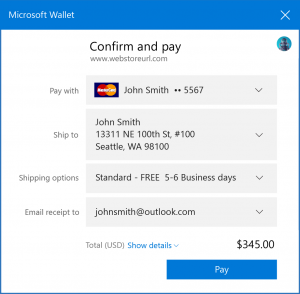
\includegraphics[width=1\linewidth]{wallet1}
		\caption{Wallet dopo la chiamata request.show()}
		\label{fig: Wallet dopo la chiamata request.show()}
	\end{figure}
	\begin{flushleft}
		I clienti possono quindi selezionare le informazioni di pagamento, l'indirizzo di spedizione e altri campi appropriati, quindi fare clic su Paga quando è pronto. A questo punto, gli utenti dovranno verificare la loro identità. In caso di esito positivo, ciò soddisferà la promessa request.show () e restituirà al sito Web tutte le informazioni che il cliente ha fornito al Portafoglio. Per il metodo di pagamento con carta di base, l'oggetto risultato conterrà il nome del titolare della carta, il numero della carta, il mese di scadenza e altri campi pertinenti. Il commerciante può quindi utilizzare queste informazioni per elaborare la transazione sul back-end.
		Dopo che la risposta è tornata dal server, è possibile utilizzare result.complete ('successo') per visualizzare la schermata di successo nel Portafoglio e result.complete ('fail') per indicare una transazione fallita.
	\end{flushleft}

	\pagebreak
	\begin{lstlisting}
	// Mostra l'interfaccia utente nativa
	payment.show()
	// Quando la promessa e soddisfatta, passa i risultati al tuo server per l'elaborazione
	.then(result => {
		return process(result).then(response => {
			if (response.status === 200) {
				// Mostra che la transazione ha avuto successo nell'interfaccia utente
				return result.complete('success');
			} else {
					// Mostra nell'interfaccia utente nativa che la transazione ha avuto esito negativo
					return result.complete('fail');
				}
			}).catch((err) => {
			console.error('User rejected request', err.message)
		}); 
	});
	\end{lstlisting}
	
	\begin{figure}
		\centering
		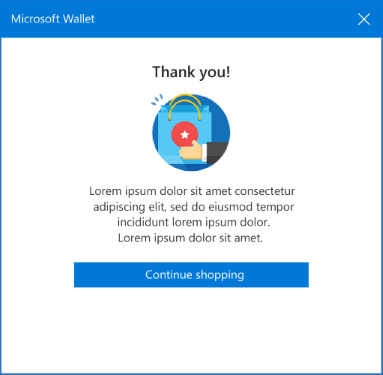
\includegraphics[width=1\linewidth]{wallet2}
		\caption{Wallet in caso di successo}
		\label{fig: Wallet in caso di successo}
	\end{figure}
	\begin{figure}
		\centering
		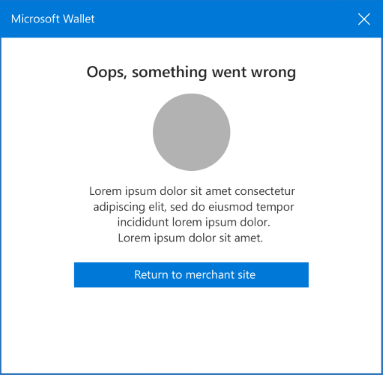
\includegraphics[width=1\linewidth]{wallet3}
		\caption{Wallet in caso di fail}
		\label{fig: Wallet in caso di fail}
	\end{figure}


	\subsubsection{Ascoltando gli eventi}
	Il prezzo potrebbe cambiare in base all'indirizzo di spedizione e alle opzioni di spedizione selezionate dal cliente. È possibile ascoltare tali modifiche con gli eventi shippingaddresschange e shippingoptionchange per ricalcolare di conseguenza i prezzi.
	\begin{lstlisting}
		payment.addEventListener("shippingaddresschange", function (changeEvent) {
			    // Elabora la modifica dell'indirizzo di spedizione
		});
		
		payment.addEventListener("shippingoptionchange", function (changeEvent) {
			// Modifica delle opzioni di spedizione del processo (ad esempio "spedizione in giornata")
		});
	\end{lstlisting}
	
	\subsubsection{Rilevamento di funzionalità}
	I siti possono essere rilevati per l'API di richiesta di pagamento, inoltrare l'utente a un'esperienza legacy, basata su moduli, se non è disponibile.
	\begin{lstlisting}
			// Inoltra utente alla verifica basata su modulo se PaymentRequest non e disponibile
			if (!window.PaymentRequest) {
				window.location.href = '/form-based-checkout';
				return;
			}
	\end{lstlisting}
	\begin{flushleft}
		Ecco un esempio di implementazione minima di questo codice:
	\end{flushleft}
	\pagebreak
	\begin{lstlisting}
	function startPaymentRequestCheckout() {
		var methodData = [
			{     
				supportedMethods: ['basic-card'],     
				data: {          
					supportedNetworks: ['visa', 'mastercard', 'amex'],
					supportedTypes: ['credit']                
				}    
			}     
		]; 
		
		var details =  {
				displayItems: [
					{
						label: "Sub-total",
						amount: { currency: "USD", value : "100.00" }, // US$100.00
					},
					{
						label: "Sales Tax",
						amount: { currency: "USD", value : "9.00" }, // US$9.00
					}
				],
				total:  {
					label: "Total due",
					amount: { currency: "USD", value : "109.00" }, // US$109.00
				}
		};
			
		var options = {
			requestShipping: true 
		};
			
		var request = new PaymentRequest(methodData, details, options);
		
		//Show the Native UI
		request.show()
		//When the promise is fulfilled, pass the results to your server for processing
		.then(result => {
			return process(result).then(response => {
				if (response.status === 200) {
					//Show that the transaction was successful in the UI
					return result.complete('success');
				} else {
					//Show in the Native UI that the transaction failed
					return result.complete('fail');
				}
			})
		});
		
		request.addEventListener("shippingaddresschange", function (changeEvent) {
			// Process shipping address change
		});
		
		request.addEventListener("onshippingoptionchange", function (changeEvent) {
			// Process shipping option change (e.g. "one day shipping")
		});
	}
	document.getElementById('#checkout').addEventListener('click', startPaymentRequestCheckout)
	\end{lstlisting}
	\section{Compatibilità web}
	\pagebreak
		\begin{figure}
			\centering
			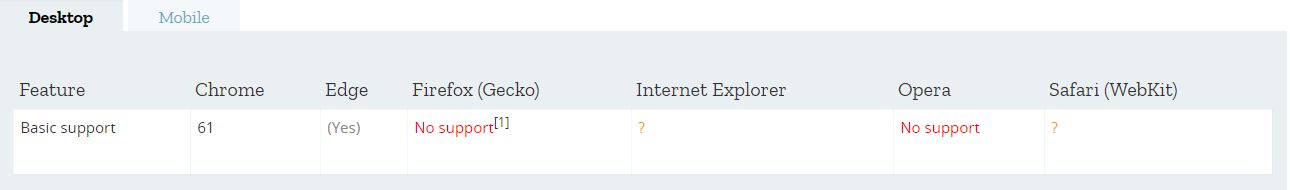
\includegraphics[width=1\linewidth]{Compatibilita1}
			\caption{Compatibilità desktop}
			\label{fig: Compatibilità desktop}
		\end{figure}
		\begin{figure}
			\centering
			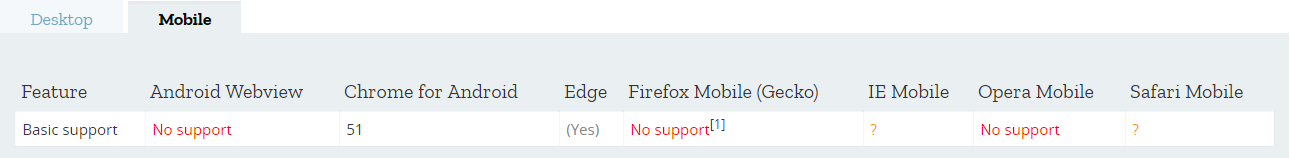
\includegraphics[width=1\linewidth]{Compatibilita2}
			\caption{Compatibilità mobile}
			\label{fig: Compatibilità mobile}
		\end{figure}
	\section{Conclusioni}
	L'API di richiesta di pagamento fornisce un potente strumento per i commercianti per migliorare la conversione del checkout sul Web e per offrire ai clienti un'esperienza di acquisto più piacevole e conveniente. Questa API è un ottimo esempio della potenza e della flessibilità della piattaforma web, ed è sulla strada per un'ampia interoperabilità, con Chrome per Android che supporta l'API a partire da Chrome 54.
\end{document}